\documentclass{standalone}
\usepackage{tikz}
\begin{document}

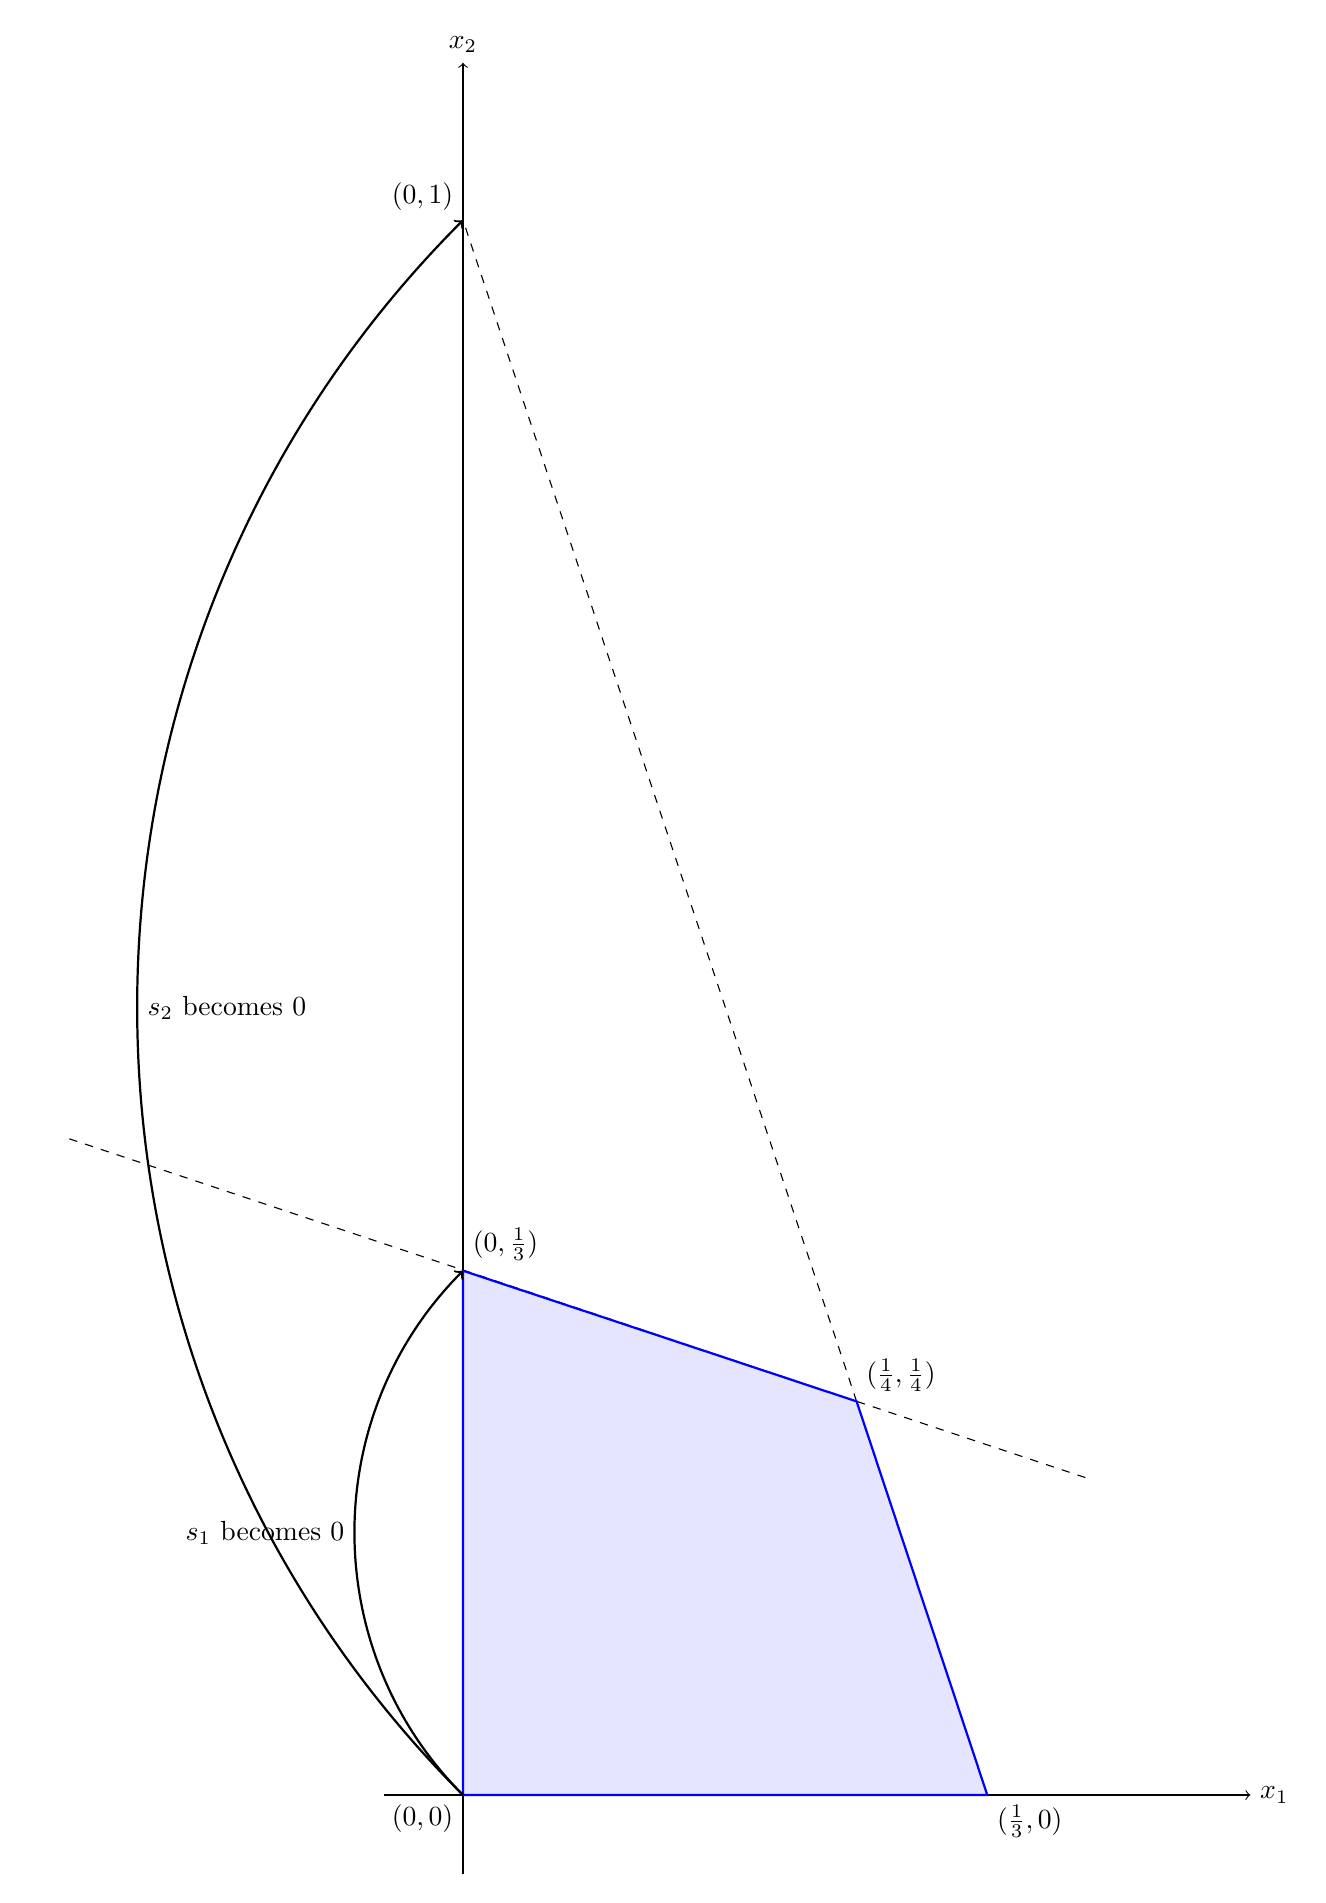
\begin{tikzpicture}[scale=20]
  % Ax_1es
  \draw[->] (-0.05, 0) -- (0.5, 0) node[right] {$x_1$};
  \draw[->] (0, -0.05) -- (0, 1.1) node[above] {$x_2$};

  % Define the points
  \coordinate (A) at (0, 0);
  \coordinate (B) at (0.333, 0);
  \coordinate (C) at (0.25, 0.25);
  \coordinate (D) at (0, 0.333);


 \draw[dashed] (-.25, .41667) -- (.4, .2);
 \draw[dashed] (C) -- (0, 1);
  % Fill the polytope
  \filldraw[fill=blue!10, draw=blue, thick]
    (A) -- (B) -- (C) -- (D) -- cycle;

  % Label the points
  \node[below left] at (A) {$(0, 0)$};
  \node[below right] at (B) {$(\frac{1}{3}, 0)$};
  \node[above right] at (C) {$(\frac{1}{4}, \frac{1}{4})$};
  \node[above right] at (D) {$(0, \frac{1}{3})$};
  \node[above left] at (0, 1) {$(0, 1)$};

  % Draw the two choices
    \draw [->, thick] (A) to [out=135, in=-135] node[midway, left]
    {$s_1$ becomes 0} (D);

    \draw [->, thick] (A) to [out=135, in=-135] node[midway, right]
    {$s_2$ becomes 0} (0, 1);
\end{tikzpicture}

\end{document}
